\documentclass[12pt]{article}

\usepackage{preamble}



%title, author, date
\title{Netzwerkanalyse mit Wireshark: Was passiert im Netzwerk?}
\author{Luis Herzog}
\date{April 2023}




\begin{document}





%Titlepage

\maketitle


\thispagestyle{empty}

\begin{figure}[h]
	\centering
	
\includegraphics[scale=0.1]{Bilder/Wireshark_icon.svg.png}
	\caption{Wireshark Logo}
	\label{fig:figure1}
\end{figure}


\newpage
\tableofcontents
\newpage

Es gibt viele verschiedenen Arten von Daten. Somit ebenfalls verschiedene Definitionen. 

Bevor man über die Wireshark Software sprechen kann, müssen die Basics geklärt werden:

\begin{itemize}
	\item Was sind Protokolle?
	\item Welche Protokolle gibt es?
	\item Wie funktionieren die Protokolle?
	\item welcche Protokolle (welche können ausgelesen werden?
\end{itemize}

\section{Daten}
\subsection{Metadaten}



\section{Das Programm: Wireshark}

Als ``Schweizer Taschenmesser``\cite{schweizer-taschenmesser} wird es von heise.de bezeichnet. Es wird so gut wie überall in der IT-Branche benutzt. Sei es beim Finden von Netzwerkproblemen oder beim Lernen, wie ein Netzwerk funktioniert. Es bietet eine Menge Möglichkeiten
\subsection{Programm}



\begin{figure}[h]
	\begin{center}
		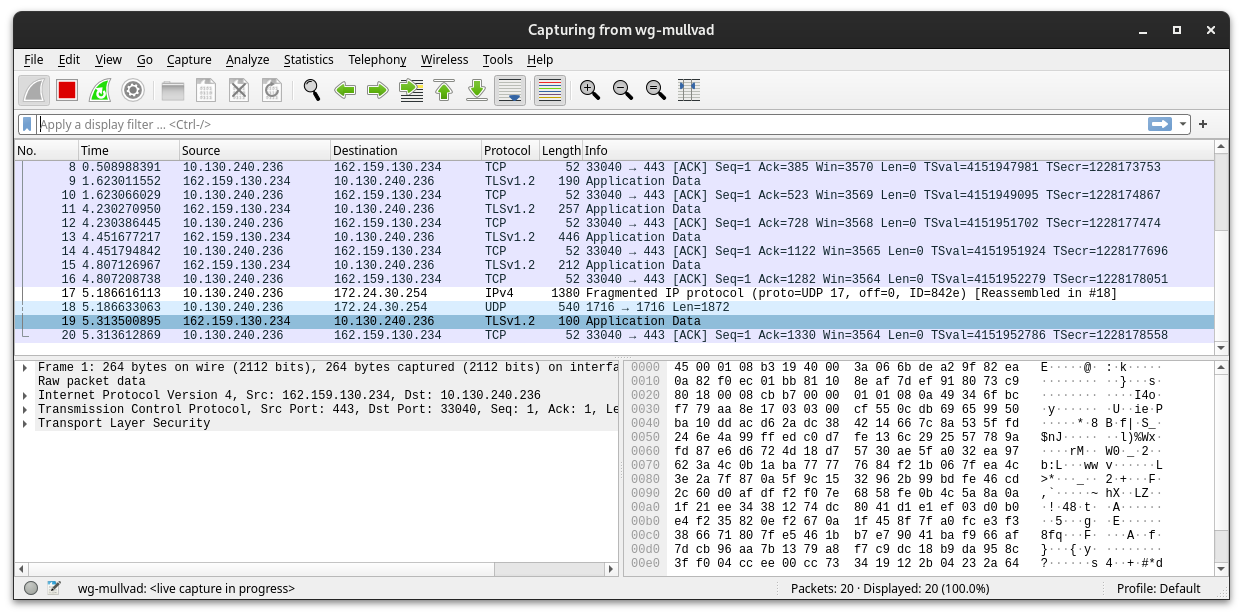
\includegraphics[scale=0.25]{Bilder/Screenshot_1.png}
		\label{fig:figure2}
		\caption{Beispielscreenshot aus der Wireshark Software}
	\end{center}
\end{figure}


\subsection{Funktionsumfang}

Wireshark ist eine Software mit sehr vielen Funktionen. Sie bietet wirklich alles rund um das Thema Netzwerkanalyse. Die wichtigsten Funktionen sind:
\begin{itemize}
	\item Die Verfügbarkeit aus sehr vielen Platformen
	\item Die Möglichkeit dumps von anderen Personen importieren zu können
	\item Das Filtern von Paketen nach sehr vielen Kriterien
\end{itemize}
Besonders die letztere Funktion ist sehr wichtig, da man ohne diese schnell die Orientierung in der Software verlieren kann. \cite{features}

\subsection{Anwendungsbereiche}
Wie im oberen Teil schon dargestellt, hat Wireshark sehr viele Funktionen. Allein deswegen wird es auch als Schweizer Taschenmesser der Netzwerktechnik bezeichnet. Somit kann Wireshark in sehr vielen Situationen Anwendung finden. Es kann beispielsweise von Netzwerk Administratoren benutzt werden, um Netzwerk Probleme  zu Analysieren und zu lösen. Es kann außerdem von den Sicherheitsanalysten eines Netzwerks benuzt werden, um Sicherheitsprobleme in Netzwerken zu finden. Wiederum kann es auch von Anwendungsentwicklern benutzt werden, um Netzwerkprotokoll Implementationen zu debuggen. Zuletzt kann es auch benutzt werden um mehr über Netzwerktraffic zu lernen und diesen zu Analysieren. Es gibt natürlich auch viele weitere Möglichkeiten Wireshark zu benutzen. \cite{intendedpurposes}

\newpage





\section{Netzwerk}

\subsection{Aufbau}
\subsection{Protokolle}
% tcp, udp, http(s), tls/ssl,  
% tor

\subsection{Open System Interconnection Modell}

\begin{wrapfigure}{r}{0pt}
	\centering
	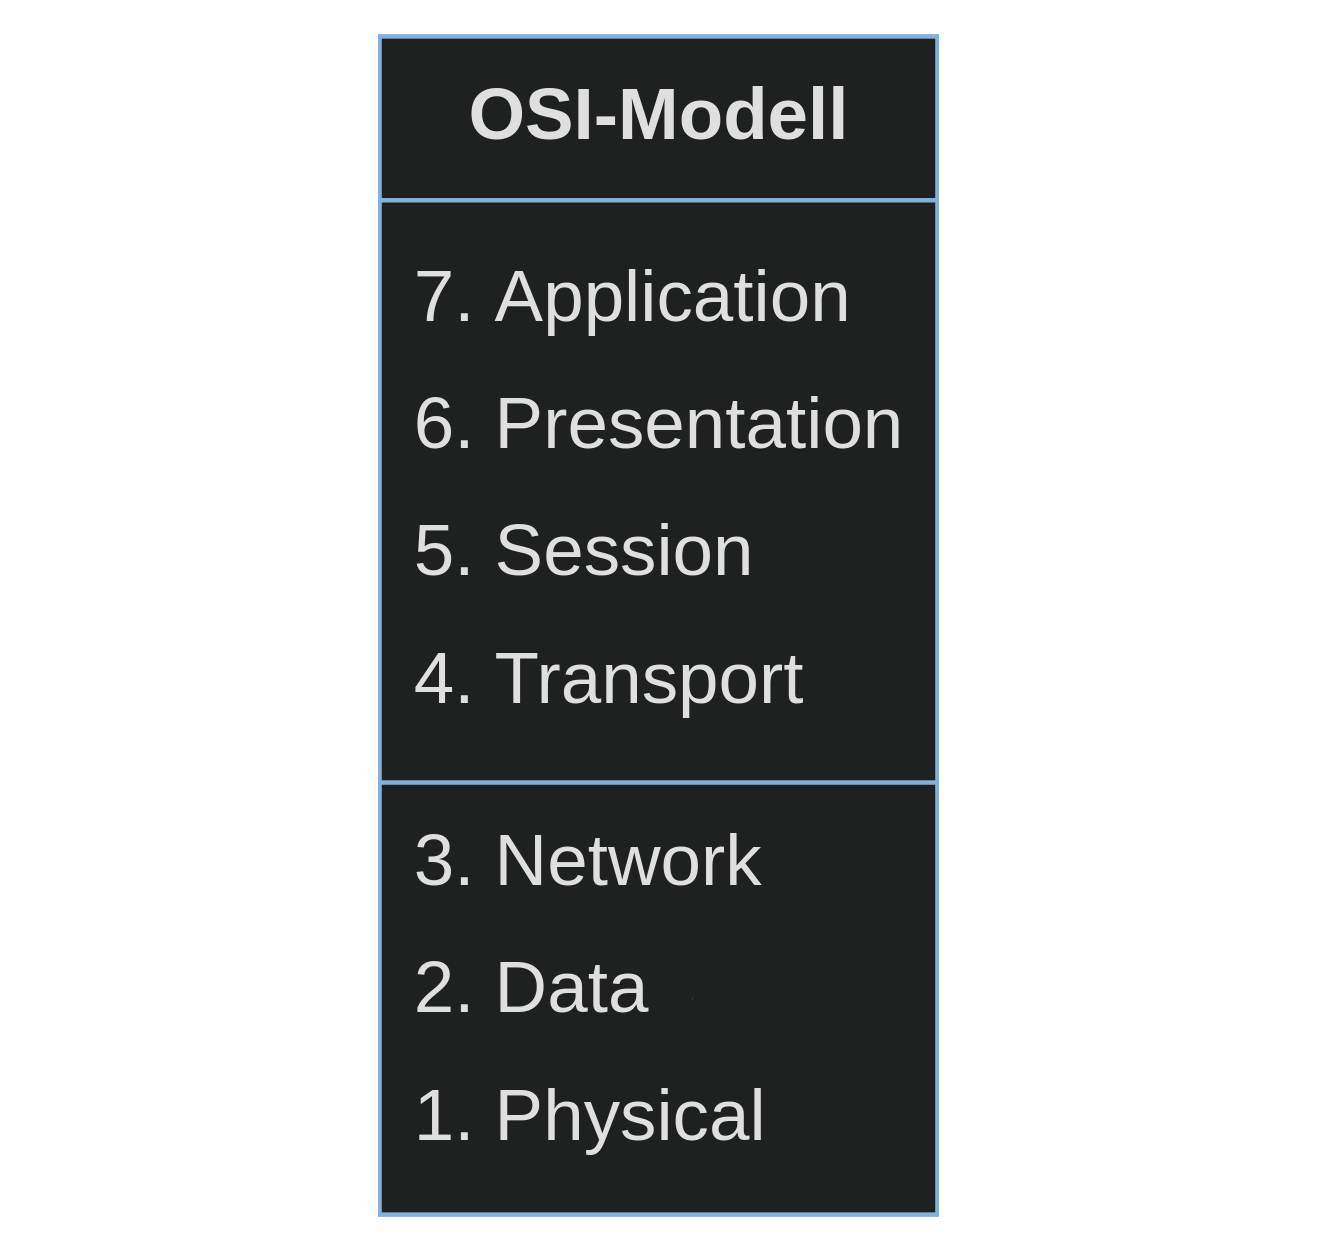
\includegraphics[scale=0.1]{Bilder/OSI-Modell}
	\caption{OSI-Modell}
	\label{fig:figure3}
	
\end{wrapfigure}

	Das Open System Interconnect\footnote{dt: Offenes System für Kommunikationsverbindungen} Modell, auch OSI-Modell genannt, beschreibt die Voraussetzungen, die für eine Kommunikation innerhalb eines Netzwerks nötig sind. Dieses wurde 1983 von durch die `Internationale Organisation für Normung`, kurz `ISO` standardisiert. Dies ist notwendig, damit sich alle Komponenten im Netwerk, auch wenn diese von verschiedenen Herstellern produziert wurden, reibungslos miteinander funktionieren. Wenn ein Paket beispielsweise von einem Computer im Netwerk losgeschickt wird, muss es mehrere Stationen durchlaufen. Das Paket verlässt den Rechner über die Netzwerkkarte und wird durch ein Übertragungsmedium über weitere Netzwerkkomponenten, wie Hubs oder Router bis zur Netzwerkkarte des Zielrechners geleitet. Dort wird dieses dann Interpretiert, um korrekt dargestellt zu werden. All diese Schritte werden durch ein Protokoll festgehalten und durch das OSI-Modell spezifiziert, damit jede Station auf diesem Weg weiß, wohin das Paket möchte, woher es kommt und welche Eigenschaften es hat. So wird ein Standart geschaffen, mit dem alle Computersysteme miteinander kommunizieren können.
	
	Da diese  Datenkommunikation relativ komplex ist, wurde das Modell in sieben Schichten eingeteilt. Die oberen vier Schichten gehören zu den Anwendungsorientierten Schichten\footnote{engl: Host layer}. Die unteren drei Schichten werden Transport Schichten\footnote{dt: Media layer} genannt. Jede Schicht behandelt eine Anforderung, die für eine funktionierende Kommunikation erfüllt werden muss. Ein zu übertragenes Paket durchläuft vor der Versendung die Schichten 7 - 2, wobei dem Paket bei jeder Schicht Protokoll-Informationen hinzugefügt werden, die dann im Protokoll des Datenpaketes auffindbar sind. Die erste und letzte Schicht wandelt das Paket in technisch übertragbare Daten um und schickt dieses über das Übertragsmedium weg. Das Übertragsmedium kann hierbei ein Kabel sein, oder aus einer Antenne bestehen. Auf der Empfängerseite wird dieser Prozess rückwärts durchgeführt. Hierbei wird die jeweilige Protokoll-Information nach der Interpretierung durch die jeweilige Schicht entfernt, bis zum Inhalt des Paketes.
	
	Im folgenden werden die einzelnen Schichten  einzeln beleuchtet, um einen besseren Einblick zu gewähren.

\subsubsection{Anwendungsschicht}
	Die Anwendungsschicht\footnote{engl: application layer} stellt die Daten dar, mit welchen der Nutzer interagiert. Softwareanwendungen, wie Web-Browser und E-Mail clients stützen sich auf die siebte Schicht, um dem Nutzer aussagekräftige Daten zu präsentieren. 
	
	Hierzu gehören Protokolle, wie HTTP\footnote{Hyper Text Transfer Protocol}, welches benutzt wird, um Websites welche in HTML\footnote{Hyper Text Markup Language} geschrieben sind zu präsentieren, oder SMTP\footnote{Simple Mail Transfer Protocol}, welches benutzt wird um E-Mails zu präsentieren.

\subsubsection{Präsentationsschicht}
	Die Präsentationsschicht\footnote{engl: presentation layer} ist in erster Linie dafür verantwortlich, die Daten so aufzubereiten, dass diese in der Anwendungsschicht verwendet werden können. Ein wichtiger Teil dabei ist die Verschlüsselung. Die Präsentationsschicht muss, wenn die Geräte durch eine verschlüsselte Verbindung kommunizieren, auf Senderseite eine Verschlüsselung hinzufügen und diese auf der Empfängerseite korrekt dekodieren. 
	
	Ebenso ist die Präsentationsschicht für die Komprimierung der Daten verantwortlich. Dadurch kann die Geschwindigkeit und Effizienz der Kommunikation erhöht und die benötigte Bandbreite minimiert werden.

\subsubsection{Sitzungsschicht}
	Anschließend folgt die Sitzungsschicht\footnote{engl: session layer}. Diese ist für das Öffnen und Schließen der Kommunikation der beiden Geräte zuständig. Hier wird die Kommunikation in Sitzungen eingeteilt. Eine Sitzung reicht von der Öffnung bis zur Schließung der Verbindung. Somit wird sicher gestellt, dass die Sitzung lange genug geöffnet bleibt, um alle Daten zu übertragen. Wenn alle Daten erfolgreich übertragen wurden, leitet die Sitzungsschicht die umgehende Schließung der Sitzung ein, um Ressourcen zu sparen. 
	
	Eine weitere sehr wichtige Aufgabe der Sitzungsschicht ist die Sicherung der Datenverbindung durch synchronisierte Checkpoints. Wenn beispielsweise bei der Übertragung einer 450 Megabyte großen Datei bei 234 Megabyte die Verbindung unterbrochen wird, kann nach einer Neuverbindung die Übertragung bei 230 Megabyte wieder aufgenommen werden, da es einen Checkpoint der Datei bei 230 Megabyte gibt.

\subsubsection{Transportschicht}
	In der Transportschicht\footnote{engl: transport layer} werden die Datenpakete vor dem Versenden in Segmente zerlegt. Im Empfangsgerät werden die diese Segmente durch die Transportschicht wieder korrekt zusammengesetzt, sodass diese von der Sitzungsschicht benutzt werden können. 
	
	Die Transportebene ist ebenfalls für die Fluss- und Fehlersteuerung zuständig. Hierbei wird die Übertragungsgeschwindigkeit so festgelegt, dass ein ggf. langsamer Empfänger nicht durch die ggf. schnelle Geschwindigkeit des Senders überfordert wird. Beim Empfänger wird durch die Fehlersteuerung ein vollständiger Empfang aller Daten sichergestellt. Wenn die empfangenen Daten nicht vollständig sind, werden diese durch dieses System erneut angefordert, um die Vollständigkeit der Daten zu garantieren. 
	
	Hierzu gehören die Protokolle TCP\footnote{Transmission Control Protocol} und UDP\footnote{User Datagram Protocol}

\paragraph{Exkurs: UDP/TCP}
   
   
\subsubsection{Netzwerkschicht}
	Darauf folgt die Netzwerkschicht\footnote{engl: network layer}. Diese gewährt das Kommunizieren zwischen Geräten in verschiedenen, miteinander verbundenen Netzwerken. Beim Versenden, werden die Segmente der Transportschicht erneut in kleinere Datenpakete aufgeteilt und mit weiteren Informationen versehen. Diese Informationen sind für die, auf dem Weg gelegenen, Knoten gedacht, um diesen das Ziel des Pakets aufzuweisen. Es wird der beste physikalisch mögliche Weg ausgesucht, um die Daten sicher an ihr Ziel zu bringen. Dieser Prozess wird Routing\footnote{Quelle!} genannt.
	Wenn sich beide Geräte im selben Netzwerk befinden, wird diese Ebene übersprungen. 
	
	Zu den Protokollen für diese Schicht gehören das IP\footnote{Internet Protocol}, das ICMP\footnote{Internet Control Message Protocol}, das IGMP\footnote{Internet Group Message Protocol} und die IPsec\footnote{??} Suite. Ein Beispielgerät wäre ein Router.
	
\subsubsection{Sicherungsschicht}
	Die Sicherungsschicht\footnote{engl: Data Link Layer} stellt die vorletzte Schicht dar. Diese ist der Netzwerkschicht sehr ähnlich. Der wesentliche Unterschied ist, dass die Sicherungsschicht für die Kommunikation von zwei Geräten innerhalb eines Netzwerks zuständig ist. Die Sicherungsschicht ist ebenfalls für die Fluss- und Fehlerkontrolle in der netzinternen Kommunikation zuständig. 
	
	Beispielgeräte für diese Ebene wären Bridges und Switches.

\subsubsection{Bitübertragungsschicht}
	Die unterste Schicht wird durch die Bitübertragungsschicht\footnote{engl: physical layer} dargestellt. Hier sind die Daten als Bitstrom vorhanden, eine Zeichenkette bestehend aus einen und nullen. Hier muss sich auf mehrere Konventionen geeinigt werden. Zu Beginn müssen die Gegebenheiten des Übertragungsmediums festgelegt werden. Dies betrifft die Wahl des Materials und die Funktion der einzelnen Leitungen. Ein Kabel kann beispielsweise aus Kupfer oder Glasfaser bestehen und zwei innere Leitungen haben: eine Datenleitung und eine Steuerleitung. Bei der Übertragung über Funk wird beispielsweise durch Luft übertragen. Es muss ebenfalls die Übertragungsrichtung und Geschwindigkeit festgelegt werden. Ein Kabel kann in eine Richtung\footnote{simplex}, abwechselnd in beide Richtungen\footnote{halb-duplex} oder in beide Richtungen gleichzeitig\footnote{duplex} übertragen.





\section{Analyse}
In der Analyse soll viel benutzte Software getestet werden. Ich habe mich für Web-Browser entschieden, da diese am meisten benutzt werden\footnote{QUELLE!}. Zu beginn soll die Software getestet werden. Hierfür habe ich einen simplen Test erstellt.
\subsection{Beispiel}
In diesem Beispiel wird ein Webserver erstellt und anschließend kontaktiert. Dieser Transfer wird dann durch Wireshark aufgezeichnet.
\subsubsection{Der Webserver}
Code: 

\begin{lstlisting}
	from flask import Flask
	import os
	from datetime import datetime
	
	hostName = "localhost"
	serverPort = 8080
	app = Flask(__name__)
	@app.route('/')
	def index():
	return '<p>willkommen in der http webserver demo</p>'
	@app.route('/time')
	def time():
	now = datetime.now()
	current_time = now.strftime("%H:%M:%S")
	return f'Jetzige Zeit: {current_time}'
	
	if __name__ == '__main__':
	app.run(host=hostName, port=serverPort)
\end{lstlisting}


\subsubsection{Das `loopback device`}
\subsubsection{Ergebnis}

\subsection{Browser}
\subsubsection{Mozilla Firefox}
\subsubsection{Microsoft Edge}
 \subsubsection{Mullvad Browser}
\subsubsection{Opera Browser}




 \section{Fazit}

% end of text

\newpage
 \listoffigures
\newpage
\bibliographystyle{plain}
\bibliography{gg}

\newpage

\centering
\vspace*{200pt}
\Huge{\section{Anlagen}}

\end{document}

